% This file was created by tikzplotlib v0.9.9.
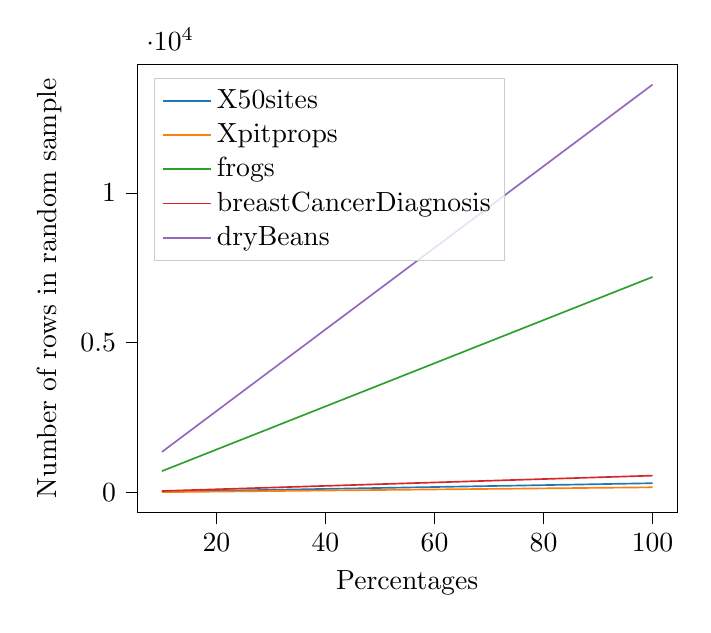
\begin{tikzpicture}

\definecolor{color0}{rgb}{0.12156862745098,0.466666666666667,0.705882352941177}
\definecolor{color1}{rgb}{1,0.498039215686275,0.0549019607843137}
\definecolor{color2}{rgb}{0.172549019607843,0.627450980392157,0.172549019607843}
\definecolor{color3}{rgb}{0.83921568627451,0.152941176470588,0.156862745098039}
\definecolor{color4}{rgb}{0.580392156862745,0.403921568627451,0.741176470588235}

\begin{axis}[
legend cell align={left},
legend style={
  fill opacity=0.8,
  draw opacity=1,
  text opacity=1,
  at={(0.03,0.97)},
  anchor=north west,
  draw=white!80!black
},
tick align=outside,
tick pos=left,
x grid style={white!69.0196078431373!black},
xlabel={Percentages},
xmin=5.5, xmax=104.5,
xtick style={color=black},
y grid style={white!69.0196078431373!black},
ylabel={Number of rows in random sample},
ymin=-661.65, ymax=14290.65,
ytick style={color=black}
]
\addplot [semithick, color0]
table {%
10 31
20 63
30 94
40 126
50 158
60 189
70 221
80 252
90 284
100 316
};
\addlegendentry{X50sites}
\addplot [semithick, color1]
table {%
10 18
20 36
30 54
40 72
50 90
60 108
70 126
80 144
90 162
100 180
};
\addlegendentry{Xpitprops}
\addplot [semithick, color2]
table {%
10 719
20 1439
30 2158
40 2878
50 3597
60 4317
70 5036
80 5756
90 6475
100 7195
};
\addlegendentry{frogs}
\addplot [semithick, color3]
table {%
10 56
20 113
30 170
40 227
50 284
60 341
70 398
80 455
90 512
100 569
};
\addlegendentry{breastCancerDiagnosis}
\addplot [semithick, color4]
table {%
10 1361
20 2722
30 4083
40 5444
50 6805
60 8166
70 9527
80 10888
90 12249
100 13611
};
\addlegendentry{dryBeans}
\end{axis}

\end{tikzpicture}
